
\texttt{InferPy} (\cite{cozar2019inferpy}) is a high-level API written in \texttt{Python} inspired by \texttt{Keras} and run on top of \texttt{Tensorflow} and \texttt{Edward} for probabilistic modeling. It is focused on enabling probabilistic modeling, flexible data processing and scalable inference.

\begin{figure}[h!]
    \centering
    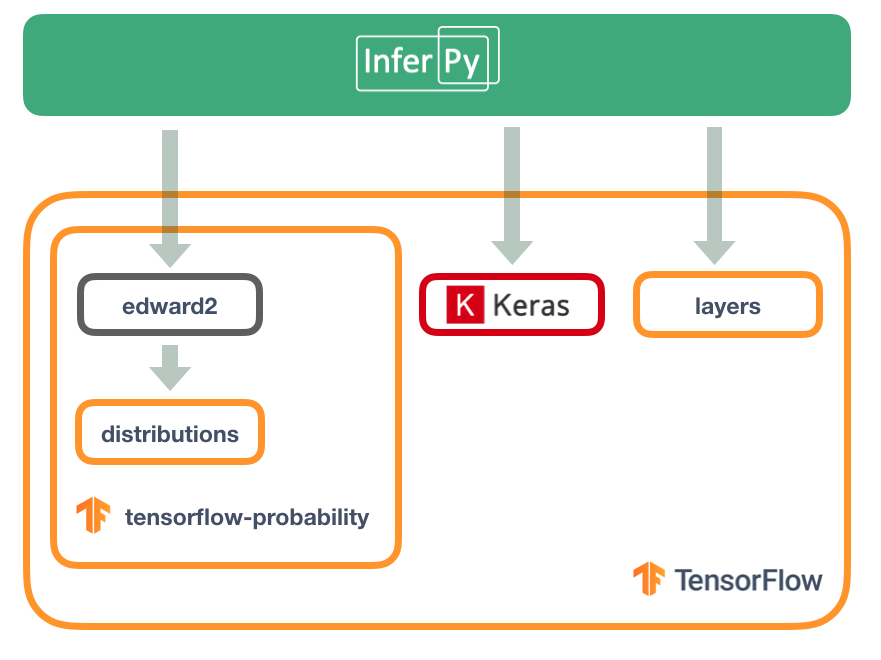
\includegraphics[width=0.7\textwidth]{tex/images/arch.png}
    \caption{InferPy architecture (\cite{cozar2019inferpy}).}
\end{figure}

\texttt{InferPy}'s main features are:
\begin{itemize}
  \item Allows to define probabilistic models whether they contain or not neural networks in a simple way.
  \item All models that can be defined using \texttt{Edward2} can also be defined in  \texttt{InferPy}, whose probability distributions are mainly inherited from \texttt{tensorflow-probability}.
  \item All the models parameters can be defined using the standard \texttt{Python} types (\texttt{Numpy} and \texttt{TensorFlow} compatibility).
  \item \texttt{InferPy} relies on top of \texttt{Edward}'s inference engine, therefore, it includes all the inference algorithms available in that package.
  \item As it uses \texttt{Edward} and \texttt{TensorFlow} as its inference engine, all the parallelization details are hidden to the user.
  \item The same code will run either in \textit{CPUs} or \textit{GPUs}.
\end{itemize}

\subsection{Installation}

\texttt{InferPy} has the following package requirements:
\begin{itemize}
    \item \texttt{Python} \( \geq\) 3.5 and \( < \) 3.8.
    \item \texttt{Tensorflow} \(\geq\)  1.12.1  and \( < \) 2.0.
    \item \texttt{Tensorflow-probability} 0.7.0.
    \item \texttt{NetworkX} \( \geq \) 2.2.0 and \( < \) 3.0.
\end{itemize}

\texttt{InferPy} is available at \texttt{Pip} and can be installed with the following command:

\begin{minted}{sh}
    pip install inferpy
\end{minted}

\subsection{Usage guide}

In all the following examples \texttt{InferPy} is imported as \texttt{inf}.

\texttt{Inferpy} requires that both the parametric \(P\) and the variational \(Q\) distribution are defined. In order to do so, models must be defined as \texttt{Python} functions inside a \texttt{@inf.probmodel} macro.

\begin{minted}{python}
    @inf.probmodel
    def model():
\end{minted}

Inside the model definition, both visible and hidden variables must be defined using the following syntax:

\begin{minted}[]{python}
    x =  inf.Normal(loc=tf.zeros([2]), scale=1, name="x")
\end{minted}

Distributions are imported from the package itself, as the case for \texttt{inf.Normal}. Distribution parameters must be passed during the definition, in this case, the mean (\texttt{loc}) and the standard deviation (\texttt{scale}) are used.

All variables must be given a name, variables with the same name in both the parametric and the variational model are considered the same variable. This is how both models communicate during the learning task. In the variational model, there must exist a parameter for each variable's parameter, in the case of the previous variable:
\begin{minted}[]{python}
    loc = inf.Parameter(tf.zeros([2]), name="x_loc")
    scale = tf.math.softplus(inf.Parameter(tf.ones([2]), name="x_scale"))
    x =  inf.Normal(loc, scale, name="x")
\end{minted}
Where a softplus function is used to avoid non-positive values.

If either the mean or the standard deviation are given as an array, a constant value on the other parameter would be interpreted as a constant array of the corresponding size. This is the case of the last definition where
\[
  X \sim \mathcal{N}_{2}(0,I).
\]

\texttt{InferPy} gives an explicit syntax for declaring a set of i.i.d random variables. Variables defined inside \texttt{with inf.datamodel(size)} are replicated the indicated number of times. This size can be omitted in the case of observations as it is calculated from the dataset at learning time.
\begin{minted}[]{python}
    with inf.datamodel():
        x = inf.Normal(tf.zeros([2]),1, name="x")
\end{minted}

When both models are defined and instantiated in a variable, we need to create an inference object, using a variational model as argument:
\begin{minted}{python}
    VI = inf.inference.VI(variational_model)
\end{minted}

By default, the inference is made using the machine learning technique \emph{gradient descent} which uses \(-\text{ELBO}\) as loss function (\href{https://github.com/PGM-Lab/InferPy/blob/master/inferpy/inference/variational/loss_functions/elbo.py}{source code}), notice that the ELBO takes values in \((-\infty, 0]\),  and uses \texttt{AdamOptimizer} (\cite{kingma2014adam}) from \texttt{TensorFlow}. An amount of \texttt{epochs} must be establish, which set the stop criteria to a of iterations to be done.

Given a training dataset \texttt{X\_train}, the model is trained indicating which set of observations corresponds to each observed variable using the following syntax:
\begin{minted}{python}
    model.fit({"x": X_train}, VI)
\end{minted}
Once the model is trained, a variable posterior can be taken as
\begin{minted}{python}
    model.posterior("z").parameters()
\end{minted}
